\section{Auswertung}
\label{sec:Auswertung}
Sämtliche im Folgenden durchgeführten Ausgleichsrechnungen werden mit der \emph{curve fit} Funktion aus dem für \emph{Python} geschriebenen package \emph{NumPy}\cite{scipy} durchgeführt. Fehlerrechnungen werden mit dem für \emph{Python} geschriebenen package \emph{Uncertainties}\cite{uncertainties} ausgeführt.

\subsection{Allgemeine Auswertung der Filmstreifen}
\label{sec:allgemein}
Für die Auswertung wurden während der Durchführung die Filmstreifen durch ein einseitiges Abschneiden der Ecken markiert, sodass im Nachhinein nachzuvollziehen ist, durch welches Loch im Filmstreifen der Röntgenstrahl eingetreten und durch welches Loch wieder ausgetreten ist. Die Markierung befindet sich an der Seite an dem der Strahl eingetreten ist. Somit wird zur Auswertung der Nullpunkt in die Mitte des Loches ohne markierten Rand gelegt, da in diesem Punkt der Strahl die Kamera verlässt. Der Abstand zwischen beiden ausgestanzten Löchern entspricht einem Winkel von $\theta=\SI{90}{\degree}$. Der Abstand der Streifen zum Nullpunkt werden mit einem Geodreieck vermessen und mit der Beziehung
\begin{align}
	\theta=\frac{s}{2R}
\end{align}
in den Beugungswinkel überführt. Dabei beschreibt $s$ den Abstand des auftretenden Reflex zum Nullpunkt und $R=\SI{5.73}{\centi\meter}$ den Radius der verwendeten Kamera.  Aufgrund der Fehleranfälligkeit beim Ablesen, wird auf jeden Reflex eine Unsicherheit  $\Delta s=\SI{1}{\milli\meter}$ angenommen.

\subsection{Metallprobe 9}
\label{sec:Metallprobe9}
Die im vorherigen Kapitel beschriebenen Messgrößen und der Netzebenenabstand $d$, welcher mit der Bragg-Bedingung \eqref{braggi} bestimmt wird, sind in Tabelle \ref{table:A1} für die verwendete Metallprobe 9 zusammengefasst.
\begin{table}
    \centering
    \caption{Messdaten der Metallprobe.}
    \label{table:A1}
    \sisetup{parse-numbers=false}
    \begin{tabular}{
	S[table-format=2.1]
	@{${}\pm{}$}
	S[table-format=1.1, table-number-alignment = left]
	S[table-format=1.3]
	@{${}\pm{}$}
	S[table-format=1.3, table-number-alignment = left]
	S[table-format=1.3]
	@{${}\pm{}$}
	S[table-format=1.3, table-number-alignment = left]
	}
	\toprule
	\multicolumn{2}{c}{$s\:/\: \si{\centi\meter}$}		& \multicolumn{2}{c}{$\theta\:/\: \si{\centi\meter}$}		&
    \multicolumn{2}{c}{$d \:/\: \si{\angstrom}$}		\\ 
	\midrule
    4.0  & 0.1 & 0.349 & 0.009 & 2.25   & 0.05   \\
5.7  & 0.1 & 0.497 & 0.009 & 1.62   & 0.03   \\
7.1  & 0.1 & 0.620 & 0.009 & 1.33   & 0.02   \\
8.4  & 0.1 & 0.733 & 0.009 & 1.15   & 0.01   \\
9.6  & 0.1 & 0.838 & 0.009 & 1.037  & 0.008  \\
10.9 & 0.1 & 0.951 & 0.009 & 0.947  & 0.006  \\
12.2 & 0.1 & 1.065 & 0.009 & 0.881  & 0.004  \\
13.8 & 0.1 & 1.204 & 0.009 & 0.826  & 0.003  \\
16.2 & 0.1 & 1.414 & 0.009 & 0.780  & 0.001  \\
16.4 & 0.1 & 1.435 & 0.009 & 0.7795 & 0.0009 \\

    \bottomrule
    \end{tabular}
    \end{table}

Die letzten beiden Einträge in der Tabelle entstehen aus einer Ringaufspaltung. Bei der Betrachtung der Netzebenenabstände $d$ für die Ringaufspaltung, ist zu erkennen, dass sich diese erst in der dritten Nachkommastelle unterscheiden. Zudem liegt der eine Wert im Fehlerintervall des anderen und umgekehrt. Aufgrund dessen werden im Folgenden die beiden Abstände gemittelt und mit der mittleren Wellenlänge der $K_\alpha$-Linie ein gemittelter Netzebenenabstand berechnet. \\

Zur Bestimmung der Kristallstruktur wird das Verhältnis
\begin{align}
	\frac{d_1}{d_i}=\frac{m_i}{m_1}
	\label{eq:dm}
\end{align}
verwendet, wobei gilt $m=\sqrt{h^2+k^2+l^2}$. Dadurch erfolgt ein Vergleich der Theorie (rechte Seite) mit den experimentell bestimmten Werten (linke Seite).
In Tabelle \ref{table:A2} sind die ersten neun Reflexe der Kristallstrukturen simple-cubic (sc), body centered cubic (bcc), face centered cubic (fcc) und Diamant aufgelistet. Zudem wird das in Gleichung \ref{eq:dm} beschriebene Verhältnis gebildet, um dieses mit der Probe zu vergleichen.

\begin{table}
    \centering
    \caption{Vergleich der Verhältnisse für die Metallprobe.}
    \label{table:A2}
    \sisetup{parse-numbers=false}
    \begin{tabular}{
	S[table-format=3.0]
	S[table-format=1.2]
	S[table-format=3.0]
	S[table-format=1.2]
	S[table-format=3.0]
	S[table-format=1.2]
	S[table-format=3.0]
	S[table-format=1.2]
	S[table-format=1.2]
	@{${}\pm{}$}
	S[table-format=1.2, table-number-alignment = left]
	}
	\toprule
	{$\text{sc}$}		& {$\left(\frac{m_i}{m_1}\right)_{sc}$}		& 
	{$\text{bcc}$}		& {$\left(\frac{m_i}{m_1}\right)_{bcc}$}		& 
	{$\text{fcc}$}		& {$\left(\frac{m_i}{m_1}\right)_{fcc}$}		& 
	{$\text{diamant}$}		& {$\left(\frac{m_i}{m_1}\right)_{dia}$}		& 
	\multicolumn{2}{c}{$\frac{d_1}{d_i}$}		\\ 
	\midrule
    100 & 1.00 & 110 & 1.00 & 111 & 1.00 & 111 & 1.00 & 1.0  & 0    \\
110 & 1.41 & 200 & 1.41 & 200 & 1.15 & 220 & 1.63 & 1.40 & 0.04 \\
111 & 1.73 & 211 & 1.73 & 220 & 1.63 & 311 & 1.91 & 1.70 & 0.05 \\
200 & 2.00 & 220 & 2.00 & 311 & 1.91 & 400 & 2.31 & 1.96 & 0.05 \\
210 & 2.24 & 310 & 2.24 & 222 & 2.00 & 331 & 2.52 & 2.17 & 0.05 \\
211 & 2.45 & 222 & 2.45 & 400 & 2.31 & 422 & 2.83 & 2.38 & 0.06 \\
220 & 2.83 & 321 & 2.65 & 331 & 2.52 & 333 & 3.00 & 2.56 & 0.06 \\
221 & 3.00 & 400 & 2.83 & 420 & 2.58 & 440 & 3.27 & 2.73 & 0.07 \\
310 & 3.16 & 330 & 3.00 & 422 & 2.83 & 531 & 3.42 & 2.90 & 0.07 \\

    \bottomrule
    \end{tabular}
    \end{table}


Die Unsicherheiten der Verhältnisse der Netzebenenabstände werden mit der Gleichung
\begin{align}
	\Delta\frac{d_1}{d_i}=\frac{d_1}{d_i}\left(\frac{\Delta d_1}{d_1} + \frac{\Delta d_i}{d_i}\right)
\end{align}
berechnet.\\
Anhand der absoluten Zahlen kann zunächst die Aussage getroffen werden, dass die Diamantstruktur nicht der gesuchten Kristallprobe entspricht. Um die anderen Strukturen bewerten zu können, wird in Tabelle \ref{table:A3} die absolute Abweichung in Prozent angegeben.

\begin{table}
    \centering
    \caption{Vergleich der Verhältnisse mit zusätzlicher Abweichung.}
    \label{table:A3}
    \sisetup{parse-numbers=false}
    \begin{tabular}{
	S[table-format=1.2]
	S[table-format=2.2]
	S[table-format=1.2]
	S[table-format=1.2]
	S[table-format=1.2]
	S[table-format=2.2]
	S[table-format=1.2]
	@{${}\pm{}$}
	S[table-format=1.2, table-number-alignment = left]
	}
	\toprule
	{$\left(\frac{m_i}{m_1}\right)_{sc}$}		& {$|Abw_{sc}|\:/\: \si{\percent}$}		& 
	{$\left(\frac{m_i}{m_1}\right)_{bcc}$}		& {$|Abw_{bcc}|\:/\: \si{\percent}$}		& 
	{$\left(\frac{m_i}{m_1}\right)_{fcc}$}		& {$|Abw_{fcc}|\:/\: \si{\percent}$}		& 
	\multicolumn{2}{c}{$\frac{d_1}{d_i}$}		\\ 
	\midrule
    1.00 & 0.00  & 1.00 & 0.00 & 1.00 & 0.00  & 1.0  & 0    \\
1.41 & 1.37  & 1.41 & 1.37 & 1.15 & 17.23 & 1.40 & 0.04 \\
1.73 & 2.01  & 1.73 & 2.01 & 1.63 & 3.82  & 1.70 & 0.05 \\
2.00 & 2.23  & 2.00 & 2.23 & 1.91 & 2.12  & 1.96 & 0.05 \\
2.24 & 2.91  & 2.24 & 2.91 & 2.00 & 7.95  & 2.17 & 0.05 \\
2.45 & 2.90  & 2.45 & 2.90 & 2.31 & 2.98  & 2.38 & 0.06 \\
2.83 & 10.60 & 2.65 & 3.46 & 2.52 & 1.59  & 2.56 & 0.06 \\
3.00 & 9.90  & 2.83 & 3.62 & 2.58 & 5.41  & 2.73 & 0.07 \\
3.16 & 9.32  & 3.00 & 3.71 & 2.83 & 2.22  & 2.89 & 0.07 \\

    \bottomrule
    \end{tabular}
    \end{table}


Zu beobachten ist, dass die bcc-Kristallstruktur kontinuierlich nur geringe Abweichungen unter $\SI{4}{\percent}$ aufweist. Somit wird angenommen, dass die Probe eine bcc-Struktur besitzt.

Des weiteren ist die Gitterkonstante $a$ der Probe zu bestimmen. Diese wird nach Gleichung \eqref{gitti} berechnet und in Abbildung \ref{fig:plot1} gegen $\cos^2{(\theta)}$ aufgetragen. Durch die verwendete lineare Ausgleichsrechnung
\begin{align}
	a(\cos{(\theta)})= b\cos^2{(\theta)} + c
	\label{eq:FIT}
\end{align}

\begin{figure}
  \centering
  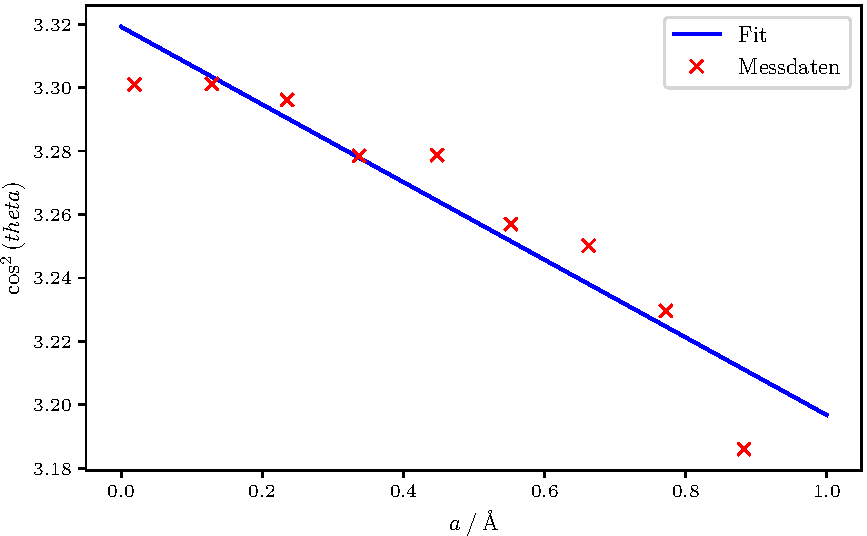
\includegraphics[scale=0.75]{build/Metall.pdf}
  \caption{Messdaten und Fitergebnis.}
  \label{fig:plot1}
\end{figure}
systematischen Fehler korrigiert. Die resultierenden Fitparameter lauten:
\begin{align}
	b&= \SI{-0.125+-0.016}{\angstrom}
 \\
	c&= \SI{3.3192+-0.0087}{\angstrom}

\end{align}

Die Gitterkonstante und die vorliegende bcc-Struktur weißt nach \cite{gitter} auf Niob hin. Die Abweichung zur der in der Literatur angegebenen Gitterkonstante
$a=\SI{3.30}{\angstrom}$ beträgt $\SI{1.038+-0.005}{\percent}
$.

\subsection{Salzprobe 5}
Die Salzprobe muss eine Gitterstruktur aufweisen, die aus zwei verschiedenen Elementen besteht. Nach \cite{skript} werden somit die Zinkblenden-, die Steinsalz, die Cäsiumchlorid- und die Fluoritstruktur im folgenden untersucht. Zuerst werden mit Gleichung \eqref{streu} alle aufkommenden Reflexe ermittelt. Da das Material unbekannt ist, lässt sich keine exakte Aussagen über den Atomformfaktor $f$ treffen, weshalb abgeschätzt werden muss, welcher der Atomformfaktoren dominiert. Somit kann nur durch starke bzw. schwache Reflexe zwischen den Gitterstrukturen unterschieden werden. In Tabelle \ref{tbl:beispieltabelle} sind die im Folgenden verwendeten Auswahlregeln zusammengefasst.

   \begin{table}
     \centering
     \caption{Auswahlregeln für verschiedene Gitterstrukturen unterteilt in Reflexe mit hoher und niedriger Intensität. Für die Steinsalz- und die Flouritstruktur gilt zusätzlich die Grundanforderung alle h,k,l gerade oder ungerade.}
     \label{tbl:beispieltabelle}
     \begin{tabular}{cc}
       \hline
       \textbf{Gittertyp}  & \textbf{Braggreflexe} \\
       \hline
       Steinsalz           & alle h,k,l ungerade und $\sum$ = 2n+1 (niedrige Intensität), sonst (hohe Intensität)     \\
       Fluorit             & alle h,k,l gerade und $\sum$ =8n+4 (niedrige Intensität), sonst (hohe Intensität)              \\
       Cäsiumchlorid       & h\:+\:k\:+\:l gerade (hohe Intensität) oder ungerade (niedrige Intensität)              \\
     \end{tabular}


     % Verweis im Text mittels \ref{tbl:beispieltabelle}

   \end{table}



   % \begin{table}
   %   \centering
   %   \caption{Auswahlregeln für verschiedene Gitterstrukturen mit Stärke der Intensität}
   %   \label{tbl:beispieltabelle}
   %   \begin{tabular}{cc}
   %     \hline
   %     \textbf{Gittertyp}  & \textbf{Braggreflexe} \\
   %     \hline
   %     Steinsalz           & alle h,k,l gerade (hohe Intensität) oder ungerade (niedrige Intensität)             \\
   %     Fluorit             & alle h,k,l gerade (hohe Intensität) oder ungerade (niedrige Intensität)              \\
   %     Cäsiumchlorid       & h\:+\:k\:+\:l gerade (hohe Intensität) oder ungerade (niedrige Intensität)              \\
   %   \end{tabular}


   %   % Verweis im Text mittels \ref{tbl:beispieltabelle}

   % \end{table}


Für die nicht aufgeführte Zinkblendenstruktur bestehen keine Auswahlregeln, weshalb die Intensitäten der zuvor bestimmten Reflexe rein rechnerisch ermittelt wird.


% werden die beiden jeweiligen Untergitter der zuvor genannten Gitterstrukturen untersucht. Tritt also ein Reflex in einem der Untergitter auf, wird dieser zu den Reflexen der Gesamtstruktur hinzugezählt. Diese Methode funktioniert nicht bei der Cäsiumchlorid-Struktur, da dessen Elementarzelle nur zwei Atome besitzt und zusätzlich einer der Koordinaten $(0,0,0)$ ist. Somit würde bei jeder Kombination von Millerindizes ein Reflex entstehen. Deshalb wird zur Vereinfachung angenommen:
% \begin{align}
% 	f_1\approx f_2
% \end{align}


Zur Identifizierung der Gitterstruktur werden wie in Kapitel \ref{sec:Metallprobe9} die theoretischen und die experimentell bestimmten Werte über das Verhältnis in Gleichung \ref{eq:dm} verglichen. Die hierfür benötigten Reflexe auf dem Filmstreifen, die sich daraus ergebenen Winkel $\theta$ und die Netzebenenabstände sind in Tabelle \ref{table:A4} aufgelistet.

\begin{table}
    \centering
    \caption{Messdaten der Salzprobe.}
    \label{table:A4}
    \sisetup{parse-numbers=false}
    \begin{tabular}{
	S[table-format=2.2]
	S[table-format=1.2]
	S[table-format=1.2]
	}
	\toprule
	{$s\:/\: \si{\centi\meter}$}		& {$\theta$}		& 
	{$d \:/\: \si{\angstrom}$}		\\ 
	\midrule
    2.75  & 0.24 & 3.24 \\
3.90  & 0.34 & 2.31 \\
4.80  & 0.42 & 1.90 \\
5.60  & 0.49 & 1.64 \\
6.30  & 0.55 & 1.48 \\
7.00  & 0.61 & 1.34 \\
8.30  & 0.72 & 1.16 \\
8.90  & 0.78 & 1.10 \\
9.55  & 0.83 & 1.04 \\
10.20 & 0.89 & 0.99 \\
11.55 & 1.01 & 0.91 \\
12.20 & 1.06 & 0.88 \\
12.80 & 1.12 & 0.86 \\
14.10 & 1.23 & 0.82 \\
14.90 & 1.30 & 0.80 \\
16.50 & 1.44 & 0.78 \\

    \bottomrule
    \end{tabular}
    \end{table}


% Da die Reflexe auf dem Filmstreifen nicht exakt zu den schwachen oder den starken Reflexen zugeordnet werden können, wird das Verhältnis $\frac{m_i}{m_1}$ auf zwei verschiedene Reflexe normiert. Dabei wird zu einen der erste starke Reflex und zum anderen der erste schwache Reflex verwendet. Die Ergebnisse der unterschiedlichen Normierungen, sowie die Markierung der starken und schwachen Reflexe sind in Abbildung \ref{fig:Anhang1} - \ref{fig:Anhang6} aufgelistet. Der schlussendliche Vergleich mit den experimentell bestimmen Werten zeigt, dass die geringste Abweichung bei den Strukturen Steinsalz/Fluorit (S) und Cäsiumchlorid (C) zu verzeichnen ist (auf den starken Reflex normiert). Zum genaueren Vergleich sind die Verhältnisse mit den absoluten Abweichungen bzgl. der gemessenen Werte in Tabelle \ref{table:A10} zusammengefasst.
Zum Vergleich der experimentell bestimmten Reflexe mit der Theorie wird das in Kapitel \ref{sec:Metallprobe9} beschriebene Verfahren verwendet. Die Ergebnisse dieses Vergleichs sind in Tabelle \ref{table:A10} und \ref{table:A70} für die Steinsalzstruktur und die Chäsiumchloridstruktur dargestellt, da diese die kleinsten Abweichungen aufweisen.

% \begin{table}
    \centering
    \caption{Vergleich der Verhältnisse.}
    \label{table:A10}
    \sisetup{parse-numbers=false}
    \begin{tabular}{
	S[table-format=3.2]
	S[table-format=1.2]
	S[table-format=1.2]
	S[table-format=3.2]
	S[table-format=1.2]
	S[table-format=1.2]
	S[table-format=1.2]
	}
	\toprule
	{$Miller_{S}$}		& {$\left(\frac{m_i}{m_1}\right)_{S}$}		& 
	{$|Abw_{S}|\:/\: \si{\percent}$}		& {$Miller_{C}$}		& 
	{$\left(\frac{m_i}{m_1}\right)_{C}$}		& {$|Abw_{C}|\:/\: \si{\percent}$}		& 
	{$\frac{d_1}{d_i}$}		\\ 
	\midrule
    110 & 1.00 & 1.00 & 0.00 & stark   \\
200 & 1.41 & 1.40 & 0.69 & stark   \\
211 & 1.73 & 1.71 & 1.22 & stark   \\
220 & 2.00 & 1.98 & 1.26 & stark   \\
310 & 2.24 & 2.20 & 1.72 & schwach \\
222 & 2.45 & 2.41 & 1.50 & stark   \\
400 & 2.83 & 2.79 & 1.46 & stark   \\
410 & 2.92 & 2.95 & 1.13 & schwach \\
420 & 3.16 & 3.11 & 1.54 & stark   \\
421 & 3.24 & 3.27 & 0.90 & schwach \\
430 & 3.54 & 3.56 & 0.64 & schwach \\
511 & 3.67 & 3.68 & 0.15 & schwach \\
432 & 3.81 & 3.78 & 0.70 & schwach \\
440 & 4.00 & 3.97 & 0.86 & stark   \\
522 & 4.06 & 4.05 & 0.19 & schwach \\
531 & 4.18 & 4.17 & 0.28 & schwach \\

    \bottomrule
    \end{tabular}
    \end{table}


% Da die Abweichungen in ähnlich kleinen Intervallen liegen, ist für eine genaue Aussage in Tabelle \ref{table:A10} der Mittelwert der absoluten Abweichungen sowie die Standardabweichung dargestellt. Auf Grundlage dieser Ergebnisse wird vorerst angenommen, dass die Probe eine Cäsiumchlorid-Struktur besitzt. 

% \begin{table}
    \centering
    \caption{Vergleich der Mittelwerte und Standardabweichungen.}
    \label{table:A11}
    \sisetup{parse-numbers=false}
    \begin{tabular}{
	l
	S[table-format=1.2]
	S[table-format=1.2]
	}
	\toprule
	{Strukturen}		& {$\text{Mittelwert}\:/\: \si{\percent}$}		& 
	{$\text{Standardabweichung}\:/\: \si{\percent}$}		\\ 
	\midrule
    Steinsalz/Fluorit & 1.02 & 0.61 \\
Cäsiumchlorid     & 0.88 & 0.57 \\

    \bottomrule
    \end{tabular}
    \end{table}


\begin{table}
    \centering
    \caption{Vergleich der Verhältnisse.}
    \label{table:A10}
    \sisetup{parse-numbers=false}
    \begin{tabular}{
	S[table-format=3.2]
	S[table-format=1.2]
	S[table-format=1.2]
	S[table-format=3.2]
	S[table-format=1.2]
	S[table-format=1.2]
	S[table-format=1.2]
	}
	\toprule
	{$Miller_{S}$}		& {$\left(\frac{m_i}{m_1}\right)_{S}$}		& 
	{$|Abw_{S}|\:/\: \si{\percent}$}		& {$Miller_{C}$}		& 
	{$\left(\frac{m_i}{m_1}\right)_{C}$}		& {$|Abw_{C}|\:/\: \si{\percent}$}		& 
	{$\frac{d_1}{d_i}$}		\\ 
	\midrule
    110 & 1.00 & 1.00 & 0.00 & stark   \\
200 & 1.41 & 1.40 & 0.69 & stark   \\
211 & 1.73 & 1.71 & 1.22 & stark   \\
220 & 2.00 & 1.98 & 1.26 & stark   \\
310 & 2.24 & 2.20 & 1.72 & schwach \\
222 & 2.45 & 2.41 & 1.50 & stark   \\
400 & 2.83 & 2.79 & 1.46 & stark   \\
410 & 2.92 & 2.95 & 1.13 & schwach \\
420 & 3.16 & 3.11 & 1.54 & stark   \\
421 & 3.24 & 3.27 & 0.90 & schwach \\
430 & 3.54 & 3.56 & 0.64 & schwach \\
511 & 3.67 & 3.68 & 0.15 & schwach \\
432 & 3.81 & 3.78 & 0.70 & schwach \\
440 & 4.00 & 3.97 & 0.86 & stark   \\
522 & 4.06 & 4.05 & 0.19 & schwach \\
531 & 4.18 & 4.17 & 0.28 & schwach \\

    \bottomrule
    \end{tabular}
    \end{table}


\begin{table}
    \centering
    \caption{Vergleich mit der Steinsalzstruktur.}
    \label{table:A70}
    \sisetup{parse-numbers=false}
    \begin{tabular}{
	S[table-format=3.0]
	S[table-format=1.2]
	S[table-format=1.2]
	S[table-format=1.2]
	l
	}
	\toprule
	{$Miller$}		& {$\left(\frac{m_i}{m_1}\right)$}		& 
	{$\frac{d_1}{d_i}$}		& {$|Abw|\:/\: \si{\percent}$}		& 
	{$Art$}		\\ 
	\midrule
    200 & 1.00 & 1.00 & 0.00 & stark   \\
220 & 1.41 & 1.40 & 0.68 & stark   \\
222 & 1.73 & 1.71 & 1.21 & stark   \\
400 & 2.00 & 1.98 & 1.26 & stark   \\
420 & 2.24 & 2.20 & 1.72 & stark   \\
422 & 2.45 & 2.41 & 1.48 & stark   \\
440 & 2.83 & 2.79 & 1.44 & stark   \\
442 & 3.00 & 2.95 & 1.73 & stark   \\
620 & 3.16 & 3.11 & 1.53 & stark   \\
622 & 3.32 & 3.27 & 1.45 & stark   \\
640 & 3.61 & 3.56 & 1.34 & stark   \\
642 & 3.74 & 3.68 & 1.69 & stark   \\
553 & 3.84 & 3.78 & 1.57 & schwach \\
555 & 4.33 & 3.97 & 9.18 & schwach \\
644 & 4.12 & 4.05 & 1.69 & stark   \\
660 & 4.24 & 4.17 & 1.71 & stark   \\

    \bottomrule
    \end{tabular}
    \end{table}


Die obigen Tabellen zeigen, dass für beiden Strukturen die Abweichungen in den selben Größenordnungen liegen, jedoch unter Verwendung der Steinsalzstruktur fast ausschließlich starke Reflexe nachgewiesen werden konnten. Dies lässt drauf schließen, dass die Salzprobe eine Steinsalzstruktur besitzt.


Wie in Kapitel \ref{sec:Metallprobe9} wird im folgenden die Gitterkonstante $a$ mit Hilfe von Gleichung \eqref{gitti} bestimmt und in Abbildung \ref{fig:SalzC} aufgetragen. Die Fitparameter der verwendeten Ausgleichsfunktion (siehe \ref{eq:FIT}) lauten:


\begin{figure}
  \centering
  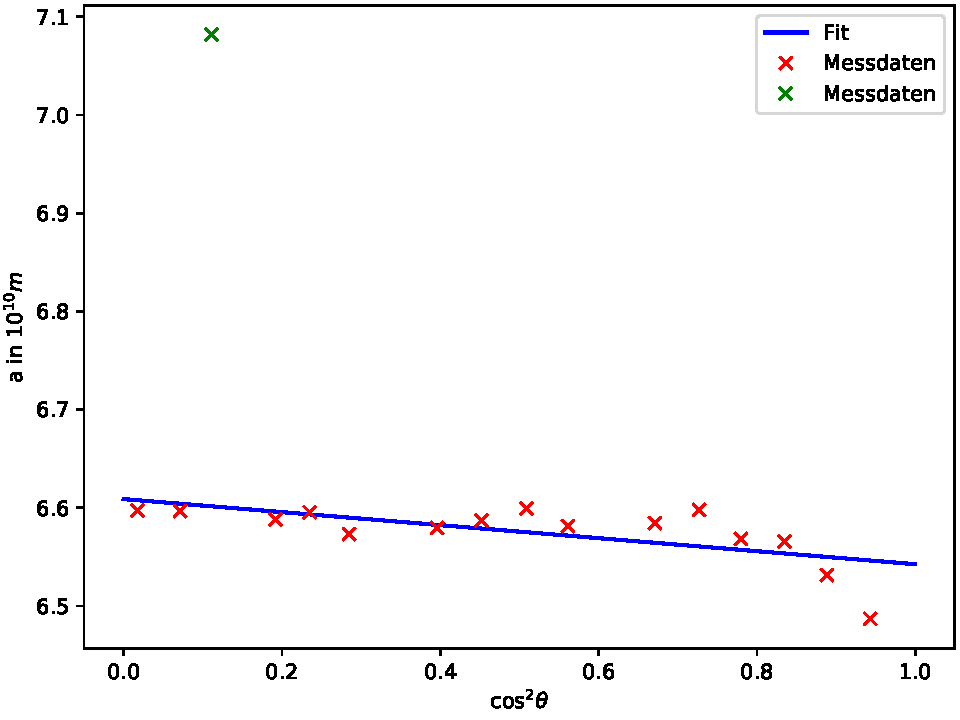
\includegraphics[scale=0.75]{build/Salz_lasttry.pdf}
  \caption{Messdaten und Fitergebnis unter der Annahme einer Steinsalz-Struktur.}
  \label{fig:SalzC}
\end{figure}


\begin{align}
	b&= \SI{-0.066+-0.021}{\angstrom}
 \\
	c&= \SI{4.579+-0.025}{\angstrom}

\end{align}

% Der nicht lineare Verlauf der Messdaten lässt auf einen Irrtum in der Zuweisung der Struktur schließen. Wird die Gitterkonstante $a$ mit der Annahme bestimmt, dass eine Steinsalz/Fluorit-Struktur vorliegt, besteht wie in Abbildung \ref{fig:SalzC2} zu sehen der erwartete linearer Zusammenhang. Die dazugehörigen Fitparameter lauten:

% \begin{figure}
%   \centering
%   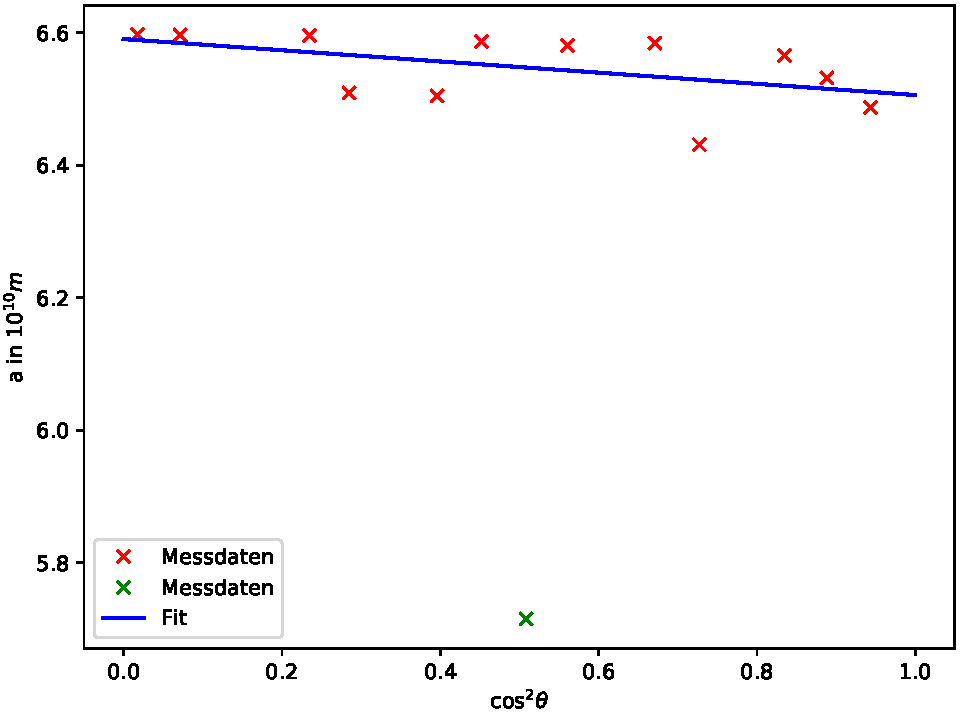
\includegraphics[scale=0.75]{build/Salz_3.pdf}
%   \caption{Messdaten und Fitergebnis unter der Annahme einer Steinsalz/Fluorit-Struktur.}
%   \label{fig:SalzC2}
% \end{figure}

% \begin{align}
% 	b&= \SI{-0.085+-0.047}{\angstrom}
 \\
% 	c&= \SI{6.590+-0.028}{\angstrom}

% \end{align}

Der in der Abbildung grün markierte Messpunkt wird als zufälliger Ausreißer behandelt und geht somit nicht in die lineare Ausgleichsrechnung mit ein. Die Ursache für diesen Messwert könnte beispielsweise eine Verunreinigung in der Salzprobe sein oder ein nicht korrekt zugeordneter Reflex. Schon in Tabelle \ref{table:A10} ist dieser Messwert auffällig, da dieser eine Abweichung von \SI{9.18}{\percent} aufweist.

Unter der Annahme, dass die Probe eine Steinsalz besitzt, ergibt sich eine Abweichung der Gitterkonstante von $\SI{-4.8+-0.4}{\percent}
$ zum Literaturwert \cite{Kaliumchlorid} von Kaliumchlorid.



% Zur Auswertung wird für jeweils alle dreizehn Reflexe auf dem Filmstreifen  und alle möglichen Millerindizes die Gitterkonstante $a$ berechnet. Stimmt die angenommene Gitterstruktur mit der Gitterstruktur der Probe überein, ist die Gitterkonstante $a$ in einer Diagonale durchgehend zu finden. Da die Zinkblenden-, die Steinsalz  und Fluoritstruktur die gleichen Reflexe aufweisen, sind diese zusammen in Abbildung \ref{fig:C_excel} und die  Cäsiumchloridstruktur in Abbildung \ref{fig:A_excel} dargestellt.

% \begin{figure}
% 	\centering
% 	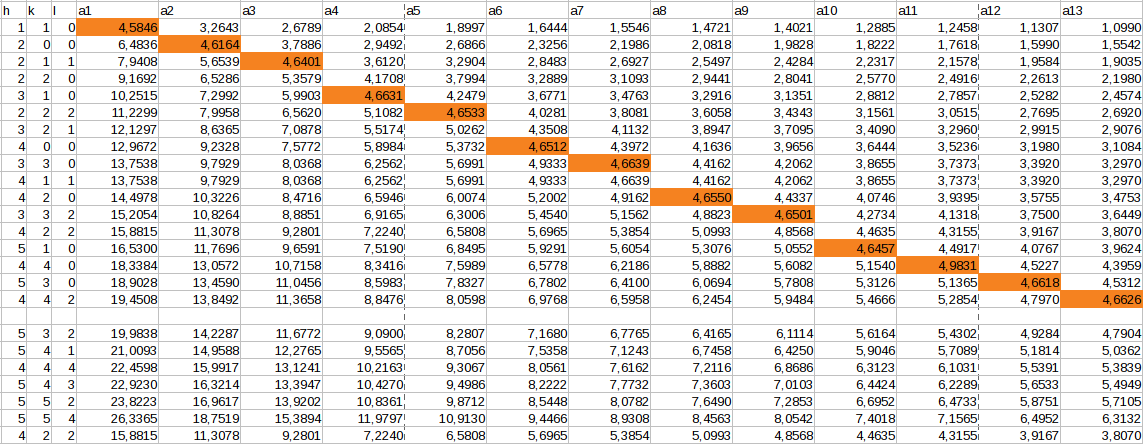
\includegraphics[angle=90,scale=0.75]{ressources/Caesiumchlorid.png}
% 	\caption{Messdaten und Fitergebnis.}
%     \label{fig:C_excel}
% \end{figure}


% \begin{figure}
% 	\centering
% 	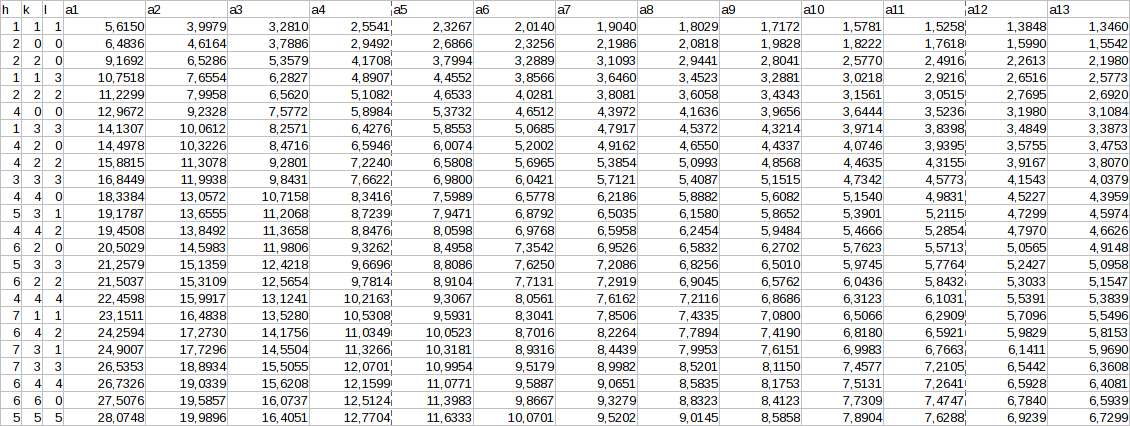
\includegraphics[angle=90,scale=0.75]{ressources/Strukturen.png}
% 	\caption{Messdaten und Fitergebnis.}
%     \label{fig:A_excel}
% \end{figure}

% Bei dem Vergleich von Abbildung \ref{fig:C_excel} und \ref{fig:A_excel} ist zuerkennen, dass die Salzprobe eine Cäsiumchloridstruktur besitzt. Zur Korrektur der systematischen Fehler wird erneut die Gitterkonstante $a$ gegen $\cos^2{\theta}$ aufgetragen und eine lineare Ausgleichsrechung \eqref{eq:FIT} vorgenommen. Es ist anzumerken, dass der in Abbildung \ref{fig:plot5} grün markierte Messwert nicht in die lineare Ausgleichrechnung eingeht.

% \begin{figure}
% 	\centering
% 	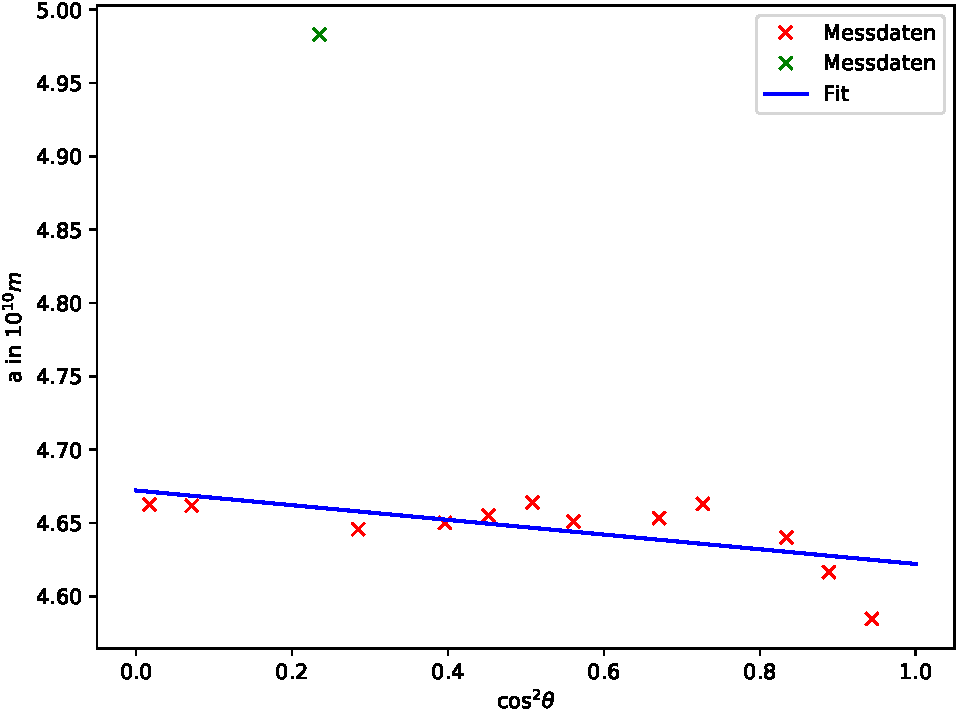
\includegraphics[scale=0.75]{build/Salz.pdf}
% 	\caption{Messdaten und Fitergebnis.}
%     \label{fig:plot5}
% \end{figure}

% Die Ergebnisse der Fitparamter lauten:

% \begin{align}
% 	b&= \SI{-0.050+-0.019}{\angstrom}
 \\
% 	c&= \SI{4.672+-0.011}{\angstrom}

% \end{align}
% Somit ist $a=\SI{4.672+-0.011}{\angstrom}
$ die experimentell bestimmte Gitterkonstante für die Salzprobe 5.

% Die experimentell bestimmte Gittekonstante $a$ und die Cäsiumchloridstruktur weisen nach \cite{CsJ} auf Caesiumiodid hin. Die Abweichung bzgl. zum Literaturwert von $a=\SI{4.56}{\angstrom}$ ergibt somit eine Abweichung von $\SI{2.46}{\percent}$.
%%%%%%%%%%%%%%%%%%%%%%%%%%%%%%%%%%%%%%%%%%%%%%%%%%%%%%%%%%%%%%%%%%%%%%%%%%%%%%%%%%%%%%%%%%%%%%%%%%%%%%%%%%%%%%%%%%%%%%%%%%%%%%%%%%%%%%%%%%%%%%%%%%%%%%%%%%%%%%%%%%


% % Examples
% \begin{equation}
%   U(t) = a \sin(b t + c) + d
% \end{equation}
%
% \begin{align}
%   a &= \input{build/a.tex} \\
%   b &= \input{build/b.tex} \\
%   c &= \input{build/c.tex} \\
%   d &= \input{build/d.tex} .
% \end{align}
% Die Messdaten und das Ergebnis des Fits sind in Abbildung~\ref{fig:plot} geplottet.
%
% %Tabelle mit Messdaten
% \begin{table}
%   \centering
%   \caption{Messdaten.}
%   \label{tab:data}
%   \sisetup{parse-numbers=false}
%   \begin{tabular}{
% % format 1.3 bedeutet eine Stelle vorm Komma, 3 danach
%     S[table-format=1.3]
%     S[table-format=-1.2]
%     @{${}\pm{}$}
%     S[table-format=1.2]
%     @{\hspace*{3em}\hspace*{\tabcolsep}}
%     S[table-format=1.3]
%     S[table-format=-1.2]
%     @{${}\pm{}$}
%     S[table-format=1.2]
%   }
%     \toprule
%     {$t \:/\: \si{\milli\second}$} & \multicolumn{2}{c}{$U \:/\: \si{\kilo\volt}$\hspace*{3em}} &
%     {$t \:/\: \si{\milli\second}$} & \multicolumn{2}{c}{$U \:/\: \si{\kilo\volt}$} \\
%     \midrule
%     \input{build/table.tex}
%     \bottomrule
%   \end{tabular}
% \end{table}
%
% % Standard Plot
% \begin{figure}
%   \centering
%   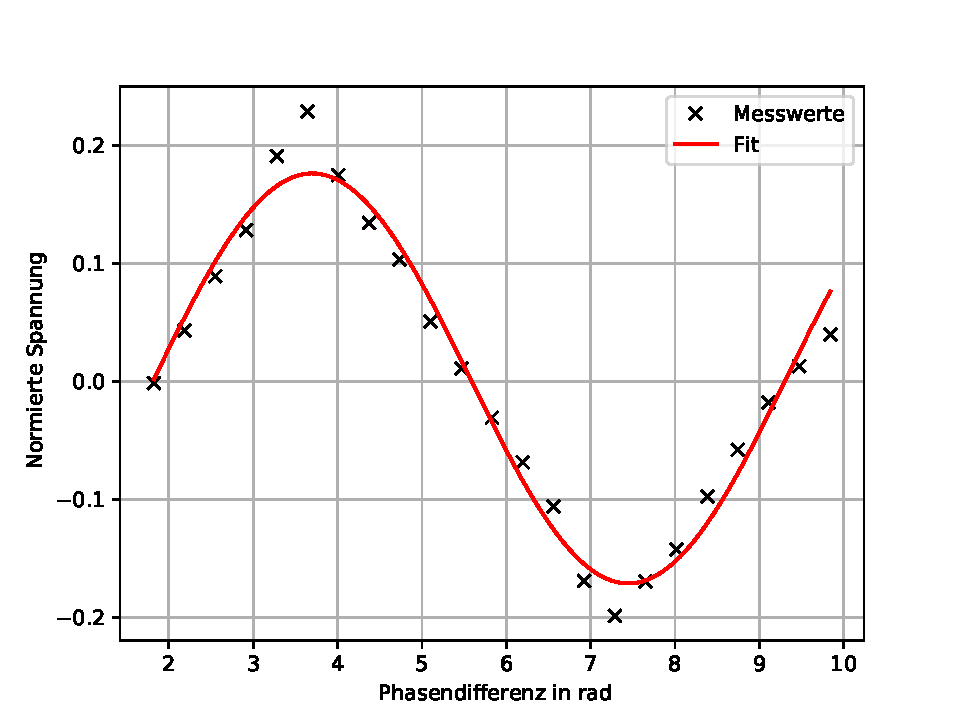
\includegraphics{build/plot.pdf}
%   \caption{Messdaten und Fitergebnis.}
%   \label{fig:plot}
% \end{figure}
%
% 2x2 Plot
% \begin{figure*}
%     \centering
%     \begin{subfigure}[b]{0.475\textwidth}
%         \centering
%         \includegraphics[width=\textwidth]{Abbildungen/Schaltung1.pdf}
%         \caption[]%
%         {{\small Schaltung 1.}}
%         \label{fig:Schaltung1}
%     \end{subfigure}
%     \hfill
%     \begin{subfigure}[b]{0.475\textwidth}
%         \centering
%         \includegraphics[width=\textwidth]{Abbildungen/Schaltung2.pdf}
%         \caption[]%
%         {{\small Schaltung 2.}}
%         \label{fig:Schaltung2}
%     \end{subfigure}
%     \vskip\baselineskip
%     \begin{subfigure}[b]{0.475\textwidth}
%         \centering
%         \includegraphics[width=\textwidth]{Abbildungen/Schaltung4.pdf}    % Zahlen vertauscht ... -.-
%         \caption[]%
%         {{\small Schaltung 3.}}
%         \label{fig:Schaltung3}
%     \end{subfigure}
%     \quad
%     \begin{subfigure}[b]{0.475\textwidth}
%         \centering
%         \includegraphics[width=\textwidth]{Abbildungen/Schaltung3.pdf}
%         \caption[]%
%         {{\small Schaltung 4.}}
%         \label{fig:Schaltung4}
%     \end{subfigure}
%     \caption[]
%     {Ersatzschaltbilder der verschiedenen Teilaufgaben.}
%     \label{fig:Schaltungen}
% \end{figure*}
